\chapter{Registration API}


\section{Goal}

MIPS\footnote{Medical Image Processing and Simulation} is a set of tools (C++ libraries and executables) offering a suite of functionalities for processing and visualizing medical images and geometric meshes. The image registration tools, which now represent a major part of MIPS, have been developed for years by the different members of the Epidaure and Asclepios teams. Due to different causes (multiple image formats, evolution of registration technics, etc.) it is quite hard to compare two methods. For the same reasons, using two different methods into a registration workflow or simply switch from one method to another one is a complicated task. At best, one usually has to write huge and complex conversion procedures which is not trivial and is very time consuming. The goal of the registration API\footnote{Application Programming Interface} is to address these issues by proposing a simple an intuitive interface shared by all registration methods. This common interface greatly simplifies the user experience while helping the author of a new registration method to focus on the algorithm, not on the user interface. We call this interface RPI for \textit{Registration Programming Interface}.


\section{RPI Specifications}



\subsection{\texttt{RegistrationMethod} class}


RPI defines a C++ programming class named \texttt{RegistrationMethod}. This class gives to a method author a strict but simple programming framework. The \texttt{RegistrationMethod} class is an abstract class and does not allow to register images. Its purpose is to provide a common interface which has been designed to cover most of registration methods. In this section, we will briefly present the \texttt{RegistrationMethod} class and its key features. The presented code has been intentionally simplified to clarify the explanation. One should read the source code for a complete and accurate specification of RPI.
\\

\texttt{RegistrationMethod} is a templated class:
\\
%
\begin{lstlisting}
template < class TFixedImage,
           class TMovingImage,
           class TTransformScalar > class RegistrationMethod
\end{lstlisting}
%
\texttt{TFixedImage} and \texttt{TMovingImage} respectively represent the types of the fixed and the moving image. \texttt{TFixedImage} and \texttt{TMovingImage} must be \texttt{itk::Image} objects. As you may know, \texttt{itk::Image} is templated over the the image dimension and the pixel type. Dimension is usually 3 while pixel type can be either a scalar type (e.g. \texttt{short}, \texttt{float}, etc.) or can be a \texttt{itk::Vector} for diffusion tensor images (DTI for short). Type \texttt{TTransformScalar} defines the type of the transformation parameters (e.g. type of each element of a affine transformation matrix). It should be either \texttt{float} or \texttt{double}. Some registration methods support different types of images and/or different types of transformation parameters (e.g. Optimus method) while other methods only support one type of images (e.g. Log-demons) or transformation parameters. In all cases, the image and transformation parameter types supported by a given registration method must clearly be stated in the code documentation. It is not of the responsibility of the user to guess the type of images and transformation parameters supported.
\\

The \texttt{RegistrationMethod} class provides all the basic necessary functions to register two images. First, the fixed and the moving images can be set and get using the following accessors:
%
\begin{lstlisting}
TFixedImage::ConstPointer  GetFixedImage(void);
void                       SetFixedImage(const TFixedImage * image);
TMovingImage::ConstPointer GetMovingImage(void);
void                       SetMovingImage(const TMovingImage * image);
\end{lstlisting}
%
Images must contain all the information necessary to orient and positioned images in the real word coordinates. One should note that the notion of smart pointer used here (\texttt{Pointer} and \texttt{ConstPointer}) is very common in ITK. The registration process can be started using the function:
%
\begin{lstlisting}
virtual void               StartRegistration(void) = 0;
\end{lstlisting}
%
As the reader may notice, this function is pure virtual since this class is only meant to be inherited. Once the registration process is complete, one can get the output transformation using the function:
%
\begin{lstlisting}
TransformPointerType       GetTransformation(void) const;
\end{lstlisting}
%
where
%
\begin{lstlisting}
typedef itk::Transform< TTransformScalarType,
                        TFixedImage::ImageDimension,
                        TMovingImage::ImageDimension > TransformType;
                        
typedef typename TransformType::Pointer TransformPointerType;
\end{lstlisting}
%
The computed transformation must be a transformation in the real world coordinates allowing to resample the moving image, \textit{i.e.} the transformation from the fixed image to the moving image.
\\
Images and transformations are stored into ITK containers. This choice was decided by the Asclepios team members and was justify by the following points:
%
\begin{itemize}
    \item ITK is an open-source library.
    \item The ITK code is maintained by hundreds of developers.
    \item All the registration methods recently developed by the team use ITK objects for images and transformations.
    \item The IO procedures to read/write images and transformations are provided by ITK.
    \item Most of image format are supported by ITK.
    \item ITK provides useful tools to manipulate images and transformations.
\end{itemize}
%
Any transformation computed by any registration method of RPI must inherit from the \texttt{itk::Transform} class (see section\ref{chap:transformations}).
\\

ITK also provides a registration framework and one may ask why RPI is not included into this framework. The ITK registration framework is too specific and does not allow to easily integrate few of Asclepios' registration methods such as \textit{Baladin} and \textit{SuperBaloo}. As a consequence, it has been decided not to base the registration API on this framework but to design a new framework more simple and more generic. Only the ITK containers were used for the reasons given previously.



\subsection{Creating a new registration class}


Any registration method of RPI must inherit from the super class \texttt{RegistrationMethod}. By definition, a registration method (\textit{i.e.} derived class) inherits all the necessary functions to set inputs, start registration, and get the output transformation. Most of registration methods use parameters to modify the method behavior. The parameters (class members) as well as the corresponding accessors must be implemented into the method -- derived -- class. Several registration methods share parameters such as the maximum number of iterations. In order to have methods as consistent as possible, parameters should be consistent as well (same member's name, same accessor's name). Finally, the code must be clean, should use the latest programming standards, and must be well documented (doxygen style).



\subsection{Libraries}

So far, most of registration methods of MIPS unfortunately can be called only using a specific executable ; one of them offered a C++ library that could eventually be used within a third party application such as MedInria. In RPI, every single registration method must be compiled into a library. By following all the specifications presented in this document (inheritance from \texttt{RegistrationMethod}, use ITK images and transformations, \textit{etc.}), a library corresponding to a given registration method (called here \texttt{MyMethod}) can then be trivially used into an external application:
%
\begin{lstlisting}
typedef MyMethod<TFixedImage,TMovingImage,TransformScalarType> Method;

MyMethod * method = new MyMethod();
method->SetFixedImage(fixed);
method->SetMovingImage(moving);
method->StartRegistration();
transform = method->GetTransformation();

// Use the transformation to do what you need to do...

delete method;
\end{lstlisting}
%
This minimal code register the two images with default parameters. To modify the method parameters, one should use the correct accessors.



\subsection{Executables}

Along with the library, each registration method must provide an executable based on its library. The executable workflow should be (more or less) the following:
%
\begin{enumerate}
\item Read input images (paths given in the command line arguments).
\item Parse method parameters from command line arguments.
\item Create a registration object.
\item Set input images and method parameters.
\item Start registration.
\item Get and save the transformation into an output file.
\item Resample the moving image using the transformation and save it into an output file.
\end{enumerate}
%
An important part of a usable executable is the parsing of the command line arguments. Among all existing tools, we propose to use the TCAL library. TCLAP provides a simple command line parser and automatically generates the usage information (``help'') using options \texttt{--help} or \texttt{-h}. The author must pay an extra attention to the description of the usage information. It is usually the only available help a user may have to learn how to correctly use a given executable.
\\

All registration executables must share the following options:
%
\begin{itemize}
\item \texttt{-f} and \texttt{--fixed-image} allows to specify the path to the fixed image.
\item \texttt{-m} and \texttt{--moving-image} allows to specify the path to the moving image.
\item \texttt{-t} and \texttt{--output-transform} allows to specify the path to the output transformation.
\item \texttt{-i} and \texttt{--output-image} allows to specify the path to the output image (moving image resampled).
\end{itemize}
%
One easily understands that since these options define the minimal input of any registration method, it becomes trivial to switch from one registration method to another one. Only advanced options must be modified.
\\

Finally, since only a single library is shared by all applications (executable and third party application), there is no duplication of the registration code. All contributors work on the same code. The code is then easier to maintain and contains necessarily less bugs. The transformation computed by an executable or by third party application (same method and same parameters) is by definition identical.



\subsection{TRex}

In order to help researchers and engineers to develop and integrate their registration method into RPI, we have developed a toy example. This example named TRex -- for \textit{Toy Registration EXample} -- is a registration method fully based on ITK. The transformation computed is a rigid transformation and the optimization method is a simple gradient descent. This example shows how to write a registration method (class) inheriting from \texttt{RegistrationMethod}, how to compile the class into a library, and how to write the code which will be compiled into a usable executable with the appropriate usage information. This example is simple, well documented and very easy to understand. The method has only one parameter.



\subsection{Observers}

Depending on the registration method, the set of parameters used, and the input images, the registration process may be very long task. If the considered method is included into an application such as MedInria, it can be very useful to know the progression of the registration process. For instance, the software is usually waiting for the process to be finished before updating the current view. Therefore, we have developed an event observer.
\\
An observer is an object which is linked to the considered registration method. When the progression of the registration process changes (\textit{e.g.} registration starts, stops, \textit{etc.}), all the observers are notified. Each notified observer does a specific task defined by the user, for instance update the current view if the registration process is finished.
\\
The observer class in RPI is named \texttt{rpi::Observer} and is based on a very simple but efficient design pattern. A user that would want to define an observer must create a class that inherits from \texttt{rpi::Observer} and implement the \texttt{Update()} method which will be called by the registration method during the notification to observers:
%
\begin{lstlisting}
template < class TFixedImage,
           class TMovingImage,
           class TTransformScalarType=double >
class MyObserver : public rpi::Observer<TFixedImage,
                                        TMovingImage,
                                        TTransformScalarType>
{
public:

  typedef rpi::RegistrationMethod<TFixedImage,
                                  TMovingImage,
                                  TTransformScalarType> Method;

  void Update(void)
  {
    if (this->m_registrationMethod->GetRegistrationStatus()==
      Method::REGISTRATION_STATUS_PROCESSING)
    {
      std::cout << "I am processing..." << std::endl;
    }
    else if (this->m_registrationMethod->GetRegistrationStatus()==
      Method::REGISTRATION_STATUS_STOP)
    {
      std::cout << "I have finished!" << std::endl;
    }
  }
};
\end{lstlisting}
%
The observer is a templated class since the observer object must contain an instance of the \texttt{rpi::RegistrationMethod} object. The signification of the templates is similar too the templates used by \texttt{rpi::RegistrationMethod}. In the example given previously, one understand what does the considered observer: the \texttt{Udpate()} method displays "I have finished!" if the registration process is finished, and "I am processing..." otherwise.
\\
To attach an observer to a registration method, simply use the \texttt{AttachObserver()} method. The class \texttt{rpi::RegistrationMethod} also provides the methods \texttt{GetRegistrationStatus()} and \texttt{SetRegistrationStatus()} which respectively gets and sets the status of the registration process. Two status are provided: \texttt{REGISTRATION\_STATUS\_PROCESSING} and \texttt{REGISTRATION\_STATUS\_STOP}. These two status represent the minimum information on the registration status one could expect. However, if a registration method provides a better granularity of the registration progression, this fineness may be used by the observer. In this case, the considered method updates a specific instance variable at each iteration of the algorithm and notify its associated observer. Then, the observers can access -- directly in the \texttt{Update()} method -- to the \textit{improved} progression status using the adapted accessor. This can be very useful for progression bar for instance.


\section{RPI methods}


In this section, we briefly present all the registration methods implemented into RPI. For a complete and accurate description of the method and of the parameters used, please refer to the corresponding code and publication (if any).



\subsection{Baladin}

Baladin~\cite{Ourselin_MICCAI_2000} is a registration method for scalar images and based on a pyramidal block-matching algorithm. Blocks are built in the moving image and, for each block, the most similar block is searched in the fixed image (exploration). Each paring of blocks defines a displacement vector. The set of displacement vector is finally used to estimate a linear transformation from the fixed to the moving image. The linear transformation computed can be a rigid transformation, a similitude, or an affine transformation.
\\
The output transformation computed by the library is represented as an \texttt{itk::\-Affine\-Transform\-<ScalarType,\-3>} object where \texttt{ScalarType} is either \texttt{float} or \texttt{double}. The output transformation computed by the executable is represented by an \texttt{itk::\-Affine\-Transform\-<double,\-3>} stored into a text file.
\\
Baladin can be initialized with a linear transformation (rigid, similitude, or affine) computed using Baladin, Baloo, or Optimus. If no initial transformation is provided, the initial transformation is simply the identity. If the type of the initial transformation is different from the type specified, the output transformation may not be of the type specified. The reason is that Baladin computes a linear transformation of the specified type that will be fused to the global transformation. For instance, if the initial transformation is the identity, the composition of rigid transformations is a rigid transformation. However, if the initial transformation is affine, the composition of affine and rigid transformations is an affine transformation.



\subsection{Optimus}

Optimus is a registration method for scalar images and based on the New UOA optimizer of Powell. The transformation computed by the registration method is a rigid transformation represented as an \texttt{itk::Euler3DTransform<double,3>} object and written into a text file for the executable. Optimus can only be initialized by an \texttt{itk::Euler3DTransform<double,3>} transformation. So far, the only registration in RPI able to compute an \texttt{itk::\-Euler3D\-Transform\-<double,\-3>} is Optimus.



\subsection{Baloo}

Baloo is a registration method for scalar and tensor images (2 classes) and based on a pyramidal block-matching algorithm. The transformation computed by the registration method is a linear transformation among rigid, similitude, or affine transformation. The output transformation computed by the library is represented as an \texttt{itk::\-Affine\-Transform\-<ScalarType,\-3>} object where \texttt{ScalarType} is either \texttt{float} or \texttt{double}. The output transformation computed by the executable is represented by an \texttt{itk::\-Affine\-Transform\-<double,\-3>} stored into a text file. Baloo cannot be initialized by any transformation.



\subsection{SuperBaloo}

Similarly to Baloo, SuperBaloo  is a registration method for scalar and tensor images (2 classes) and based on a pyramidal block-matching algorithm. However, SuperBaloo computes a displacement field transformation.
\\
The output transformation computed by the library is represented as an \texttt{itk::\-Displacement\-Field\-Transform\-<ScalarType,\-3>} object where \texttt{ScalarType} is either \texttt{float} or \texttt{double}. The executable writes the output transformation into a vector image (NifTi, Inrimage, NRRD, etc.) where values are coded as \texttt{float}. SuperBaloo cannot be initialized by any transformation.



\subsection{Diffeomorphic Demons}

Diffeomorphic demons is a registration method for scalar images and based on the demons algorithm. The difference with the classical demons is that the transformation computed -- a displacement field -- is a diffeomorphism.
\\
The output transformation computed by the library is represented as an \texttt{itk::\-Displacement\-Field\-Transform\-<ScalarType,\-3>} object where \texttt{ScalarType} is either \texttt{float} or \texttt{double}. The executable writes the output transformation into a vector image (NifTi, Inrimage, NRRD, etc.) where values are coded as \texttt{float}.
\\
The library can be initialized only by an \texttt{itk::\-Displacement\-Field\-Transform\-<SclaraType,\-3>} object. The executable can be initialized by a displacement field (vector image) or by an (ITK) linear transformation. In the case of linear transformation, the input transformation is converted into a displacement field which can initialize the corresponding library.



\subsection{Log-Demons}

Log-Demons is a registration method for scalar images and based on the demons algorithm. The difference with the classical demons is that the transformation computed is a stationary velocity field (SVF for short) and not a displacement field. This type of transformation is a convenient tool for registration since a SVF can be trivially converted into a displacement field that is a diffeomorphism.
\\
The output transformation computed by the library is represented as an \texttt{itk::\-Stationary\-Velocity\-Field\-Transform\-<ScalarType,\-3>} object where \texttt{ScalarType} is either \texttt{float} or \texttt{double}. The executable writes the output transformation into a vector image (NifTi, Inrimage, NRRD, etc.) where values are coded as \texttt{float}.
\\
The library can be initialized only by an \texttt{itk::\-Stationary\-Velocity\-Field\-Transform\-<SclaraType,\-3>} object. The executable can be initialized by a SVF (vector image) or by an (ITK) linear transformation. In the case of linear transformation, the input transformation is converted into a SVF which can initialize the corresponding library.



\subsection{Incompressible Log-Demons}

Incompressible Log-demons -- or iLogDemons for short -- is a registration method for scalar images and based on the Log-demons algorithm. The transformation computed is a stationary velocity field (SVF for short). The difference with the Log-demons is that the method accept an input mask image ; the iLogDemons adds a constraint on the computed SVF so that the volume of the zone defined into the mask is similar before and after applying the transformation.
\\
 The output transformation computed by the library is represented as an \texttt{itk::\-Stationary\-Velocity\-Field\-Transform\-<ScalarType,\-3>} object where \texttt{ScalarType} is either \texttt{float} or \texttt{double}. The executable writes the output transformation into a vector image (NifTi, Inrimage, NRRD, etc.) where values are coded as \texttt{float}.
\\
The library can be initialized only by an \texttt{itk::\-Stationary\-Velocity\-Field\-Transform\-<SclaraType,\-3>} object. The executable can be initialized by a SVF (vector image) or by an (ITK) linear transformation. In the case of linear transformation, the input transformation is converted into a SVF which can initialize the corresponding library.

\section{Image resampling}


%-------------------------------------------------------------------------------------------
\subsection{Theory}
\label{subsec:registration:resampling:theory}

Let $F$ and $M$ be respectively the fixed and the moving images. If we want to register $M$ on $F$, we want to modify $M$ so that the modified -- or transformed -- version of $M$ can be superimposed on $F$. Instinctively, one would want to estimate the transformation from $M$ to $F$ in order to apply this transformation to $M$. Well, in fact, we need the transformation from $F$ to $M$ to resample $M$ in the geometry of $F$. This is not trivial and we will try to convince you in this section.
\\
Let $\widetilde{M}$ be the resampled version of $M$ in the geometry of $F$. Theoretically, $\widetilde{M}$ and $F$ can be superimposed and then compared for diagnosis purpose for instance. First, we create an empty image $\widetilde{M}$ which has exactly the same geometrical properties of $F$ (image size, voxel size, orientation, and origin). Second, we have to fill $\widetilde{M}$ with information \textbf{taken} from image $M$. Let $(i,j,k)$ be an index (voxel coordinates) of $\widetilde{M}$ and let $(x,y,z)$ be the corresponding world coordinates. Then, let $T_{F \rightarrow M}$ be the transformation from $F$ to $M$. The value assigned to $\widetilde{M}(x,y,z)$ (world coordinates) is given by:

\begin{equation}
\widetilde{M}(x,y,z) = M(_{F \rightarrow M}(x,y,z))
\label{eq:registration:resampling:1}
\end{equation}

If the world coordinates $T_{F \rightarrow M}(x,y,z)$ are not defined on the grid of $M$, $M(_{F \rightarrow M}(x,y,z))$ is estimated by image interpolation (see section~\ref{sec:image:interpolation}).
\\
In other words, to resample $M$, we go through the voxels of $\widetilde{M}$. For each voxel of $\widetilde{M}$ we deduce the position of the corresponding voxel into $M$ using the transformation $_{F \rightarrow M}$, and then we \textbf{take} the value at this position in $M$ and assigned it to the initial position in $\widetilde{M}$.
\\

Still not convince? Let's see now what would happen if we had the transformation $T_{M \rightarrow F}$ from $M$ to $F$. As before, we first create an empty image $\widetilde{M}$ which has exactly the same geometrical properties of $F$. We go through $M$ and for each voxel of $M$, we send its corresponding value to $\widetilde{M}$ using $T_{M \rightarrow F}$. If $(x,y,z)$ is the world coordinates of a voxel of $M$, we have:

\begin{equation}
\widetilde{M}(T_{M \rightarrow F}(x,y,z)) = M(x,y,z)
\label{eq:registration:resampling:2}
\end{equation}

First difficulty here, if coordinates $T_{M \rightarrow F}(x,y,z)$ are not defined on the grid of $\widetilde{M}$, how to assign -- or distribute -- the value $M(x,y,z)$ in $\widetilde{M}$? For the next problem, let us assume that coordinates $T_{M \rightarrow F}(x,y,z)$ are always defined on the grid of $\widetilde{M}$ in order to simplify the explanation. Let us consider the case where $M$ contains $n$ voxels while $F$ contains $2n$ voxels. Using the second scheme (transformation from $M$ to $F$), one understands that only half of voxels of $\widetilde{M}$ will receive a value from $M$. The other half won't be modified and consequently $\widetilde{M}$ will have "holes".


%-------------------------------------------------------------------------------------------
\subsection{\texttt{rpiResampleImage}}

The \texttt{rpiResampleImage} tool resample an input scalar image given an input transformation. The supported transformations are identity, linear transformations, displacement field transformations, and stationary velocity field transformations computed using the registration methods of RPI (but not only). The image specified using the \texttt{--geometry} option is used to set the resample image geometry. If the \texttt{--geometry} option is not used, the geometry of the resampled image will be either similar to the input image geometry if the input transformation is a linear transformation, or will be similar to the geometry of the input field is the input transformation is a displacement field or a stationary velocity field. Several image interpolation methods are proposed.

\section{Composition of transformations}



%-------------------------------------------------------------------------------------------
\subsection{Order of composition}
\label{subsec:tools:composition:order}

Let us consider two images $I_F$ and $I_M$ (resp. fixed and moving images). We want to register $I_M$ to $I_F$ and a common way to do it is to apply successively different registration methods. In this example, we use three registration methods (e.g. rigid, affine, and non-linear). First, we apply the first registration method between images $I_F$ and $I_M$. We obtain a transformation (form the fixed to the moving image) $T_1$ and an image $I_1$ ($I_M$ re-sampled in the geometry of $I_F$):

\begin{equation}
\textrm{method}_1(I_F,I_M) \rightarrow \{T_1,I_1\}
\end{equation}

Then we apply the second registration method between images $I_F$ and $I_1$. By considering the image $I_1$ instead of $I_M$, we initialize the registration process by starting the algorithm \textit{closer} to the optimal transformation. We obtain a transformation $T_2$ and an image $I_2$ ($I_1$ re-sampled in the geometry of $I_F$):

\begin{equation}
\textrm{method}_2(I_F,I_1) \rightarrow \{T_2,I_2\}
\end{equation}

Finally, we apply the third registration method between images $I_F$ and $I_2$. We obtain a transformation $T_3$ and an image $I_3$ ($I_2$ re-sampled in the geometry of $I_F$):

\begin{equation}
\textrm{method}_3(I_F,I_2) \rightarrow \{T_3,I_3\}
\end{equation}

If we assume that the successive registration processes improved the image registration, the image $I_3$ should be the image the most similar to $I_F$, then $I_2$, $I_1$, and finally $I_M$. An important issue here is that $I_3$ is the result of three consecutive re-samplings of the initial moving image $I_M$. In order to avoid the multiple approximations due to these re-samplings, one may want to re-sample only once $I_M$ using the global transformation from $I_F$ to $I_M$. However, this global transformation is not $T_3$ but the composition of $T_1$, $T_2$, and $T_3$. Indeed, $T_3$ is the transformation from $I_F$ to $I_2$ ; the image $I_M$ re-sampled using $T_3$ is probably not correctly registered onto $I_F$.
\\

Let us consider the image re-sampling of $I_M$ using $T_1$. Let $\mathbf{x}=(x,y,z)$ be a point (in the real world coordinates) in the real grid of the fixed image. The re-sampling is defined as:

\begin{equation}
I_1(\mathbf{x}) = I_M(T_1(\mathbf{x}))
\end{equation}

Now, let us now consider the image re-sampling of $I_1$ using $T_2$:

\begin{align}
I_2(\mathbf{x}) & = I_1(T_2(\mathbf{x})) \\
                & = I_M(T_1(T_2(\mathbf{x}))
\end{align}

Finally, we re-sample $I_2$ using $T_3$:

\begin{align}
I_3(\mathbf{x}) & = I_2(T_3(\mathbf{x})) \\
                & = I_1(T_2(T_3(\mathbf{x})) \\
                & = I_M(T_1(T_2(T_3(\mathbf{x}))) \\
                & \triangleq I_M( T_1 \circ T_2 \circ T_3(\mathbf{x}) ) \label{eq:composition}
\end{align}

Eq.~\ref{eq:composition} shows that the global transformation allowing to re-sample the image $I_M$ onto $I_F$ using a single global transformation $T$ which is the composition of $T_1$, $T_2$, and $T_3$:

\begin{equation}
T = T_1 \circ T_2 \circ T_3
\end{equation}



%-------------------------------------------------------------------------------------------
\subsection{Composing transformations using \texttt{rpiFuseTransformation}}

The \texttt{rpiFuseTransformation} executable is a program that allow to fuse (compose) a list of transformation into a unique transformation. Since it is not possible yet -- at least in a general case -- to store a list of transformations into a single file, we propose to store the list as a XML file. This XML lists the type of each transformation and the path to the files containing the transformations :
%
\begin{lstlisting}
<?xml version="1.0" encoding="UTF-8"?>

<listoftransformations>

    <transformation>
        <type>linear</type>
        <path>t0.txt</path>
        <invert>1</invert>
    </transformation>

    <transformation>
        <type>displacementfield</type>
        <path>t1.nii.gz</path>
        <invert>0</invert>
    </transformation>

</listoftransformations>
\end{lstlisting}
%

In this example, we have 2 transformations. The first one (denoted $T_0$) is a linear transformation stored into the text file ``t0.txt''. The second transformation (denoted $T_1$) is a displacement field stored into the -- image -- file ``t1.nii.gz''. The computed transformation is given by $T_0 \circ T_1$. Thus, the order the transformations written into the XML file is important since the composition of two transformations is usually not commutative (see section~\ref{subsec:tools:composition:order}). The XML file can contain any strictely positive number of transformations. The meaning of the different tags is:
%
\begin{itemize}
%
\item Tag \texttt{<listoftransformations>} contains a set of transformations. This tag is mandatory.
%
\item Tag \texttt{<transformation>} contains a transformation. This tag must be an element of the tag \texttt{<listoftransformations>}. This tag is mandatory.
%
\item Tag \texttt{<type>} contains the type of the considered transformation. The available types are ``linear'', ``displacemendfield'', and ``stiaionaryvelocityfield''. This tag must be an element of the tag \texttt{<transformation>}. This tag is mandatory.
%   
\item Tag \texttt{<path>} contains the path to the file containing the transformation. A displacement field or a stationary velocity field must be stored into an image file (e.g. Nifty, Analyse, etc.). This tag must be an element of the tag \texttt{<transformation>}. This tag is mandatory.
%
\item Tag \texttt{<invert>} indicates if the considered transformation has to be inverted before the fusion. The value ``1'' induces the transformation inversion ; the value ``0'' means no inversion. This tag is optional. By default, no inversion is performed.
%
\end{itemize}
%
The type of the output transformation depends on the transformations of the list. A list of linear transformations will be fused into a linear transformation. If the list contains at least one displacement field, the output transformation will be a displacement field. If the option "--force-displacement-field" is used, the ouput transformation will be a displacement field.
For now on, if the list contains linear transformations and stationary velocity fields, the computed transformation will be a displacement field. However, this will change in the near future in order to compute a unique stationary velocity field (thanks to Marco Lorenzi).
\\
One should choose the output file extension according to the transformation computed. Indeed, if the output transformation is a displacement field, only image format are supported (e.g. .nii). No checking on the file extension will be performed since the output transformation type is easily predictable.




\section{Conversion of transformations}


In this section, we present the conversion of a transformation of the voxel space into a transformation of the world space, and conversely. We first introduce in Fig.~\ref{fig:tools:conv:1} a scheme that will be useful to give an intuition of how the conversion procedure works. This array visually represent the projection of a point from one image to another one, or from coordinate system to another one. On the top are represented the fixed and the moving images and on the left hand-side are represented the voxel and the world coordinate systems. We present here two arrows representing the projection of a point from the voxel coordinates to the world coordinates (see Section~\ref{subsec:images:systems:projection}). In this section, $M_{fixed}$ and $M_{moving}$  will respectively represent the projection (4$\times$4) matrix of the fixed and moving images.

\begin{figure}[!htbp]
\centering
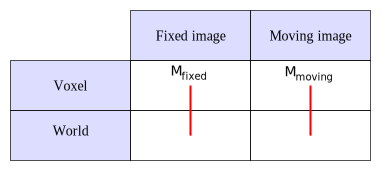
\includegraphics[width=0.5\linewidth]{conversion_transform1}
\caption{Projection matrices from the voxel coordinates to the world coordinates.}
\label{fig:tools:conv:1}
\end{figure}



%----------------------------------------------------------------------------------------------------
\subsection{Linear transformation: from voxel to world coordinates}

Let $T_{voxel}$ be a linear transformation (4$\times$4 matrix) from the fixed image to the moving image and given in the voxel coordinates (see Fig.~\ref{fig:tools:conv:2}). The conversion of $T_{voxel}$ into $T_{world}$, the corresponding linear transformation in the world coordinates, is given by:
%
\begin{equation}
T_{world} = M_{moving} . T_{voxel} . M^{-1}_{fixed}
\label{eq:tools:conv1}
\end{equation}
%
Fig.~\ref{fig:tools:conv:3} gives a visual explanation of the conversion. This conversion is used in the registration method Baloo where the initial code returns a linear transformation such as $T_{voxel}$. In the original version of Baladin, the returned transformation $T_{voxel}$ is a linear transformation from the moving image to the fixed image and given in the voxel coordinates. In this particular case, $T_{voxel}$ must be inverted before computing $T_{world}$ (from fixed to moving image) as proposed in Eq.~\ref{eq:tools:conv1}.
\\
From Eq.~\ref{eq:tools:conv1} one trivially converts a linear transformation from world coordinates to voxel coordinates:
%
\begin{equation}
T_{voxel} = M^{-1}_{moving} . T_{world} . M_{fixed}
\label{eq:tools:conv2}
\end{equation}
%
In the case of Baladin, the final transformation $T_{voxel}$ since Baladin consider transformations from the moving image to the fixed image.

\begin{figure}[!htbp]
\centering
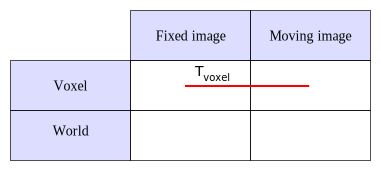
\includegraphics[width=0.5\linewidth]{conversion_transform2}
\caption{Transformation from the fixed image to the moving image and given in the voxel coordinates.}
\label{fig:tools:conv:2}
\end{figure}

\begin{figure}[!htbp]
\centering
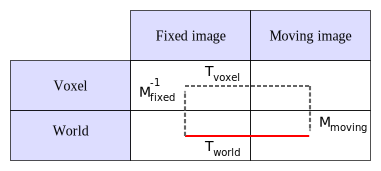
\includegraphics[width=0.5\linewidth]{conversion_transform3}
\caption{Conversion procedure: from voxel to world coordinates.}
\label{fig:tools:conv:3}
\end{figure}



%----------------------------------------------------------------------------------------------------
\subsection{Displacement field: from voxel to world coordinates}

The conversion of a displacement field is different from the conversion of a linear transformation. Indeed, a displacement vector is assigned to each element of the field. Let $p_{voxel}$ be an index of the fixed image (point in the voxel coordinates) and let $v_{voxel}$ be its associated displacement vector given in voxels. Let $p_1$ be the projection of $p_{voxel}$ into the world coordinates:
%
\begin{equation}
p_1 = M_{fixed} . p_{voxel}
\end{equation}
%
By definition, $p_{voxel} + v_{voxel}$ is an index in the moving image (point in the voxel coordinates). Let be $p_2$ be the projection of $p_{voxel} + v_{voxel}$ into the world coordinates:
%
\begin{equation}
p_2 = M_{moving} . \left( p_{voxel} + v_{voxel} \right)
\end{equation}
%
Both $p_1$ and $p_2$ are points in the world coordinates. The displacement vector, denoted $v_{world}$, in the world coordinates corresponding to $v_{voxel}$ is simply the difference between $p_2$ and $p_1$ (see Fig.~\ref{fig:tools:conv:4}):

%
\begin{equation}
v_{world} = M_{moving} . \left( p_{voxel} + v_{voxel} \right) - M_{fixed} . p_{voxel}
\end{equation}
%

\begin{figure}[!htbp]
\centering
\includegraphics[width=0.5\linewidth]{conversion_transform4}
\caption{Conversion of a displacement field from voxel to world coordinates. Green circles represent (from top to bottom and left to right) $p_{voxel}$, $p_1$, and $p_2$.}
\label{fig:tools:conv:4}
\end{figure}

\section{Other useful tools}



\subsection{\texttt{imageConvert}}

The \texttt{imageConvert} tool converts an image from one format to another. The format of each image is determined by its extension. Scalar images (2D and 3D) as well as DTI (3D) images are supported. Using some appropriate options, one can also modify the image origin, the voxel size, and the image orientation (direction). This will affect only the image header but not the content.



\subsection{\texttt{imageDisplayProperties}}

The \texttt{imageConvert} tool displays the properties of an input image. Scalar and vector images (DTI) are supported. 2D and 3D images are supported. See the example below to know what kind of information is displayed:
 
\begin{lstlisting}
[vgarcia@koch ~]$ imageDisplayProperties ~/Data/T1.nii 
Image name       : /user/vgarcia/home/Data/T1.nii
Image dimension  : 3
Image size       : [ 181, 217, 181] voxels
Pixel type       : scalar
Component number : 1
Component type   : float
Component size   : 4 bytes
Image origin     : [    0.000,    0.000,    0.000 ]
Voxel size       : [    1.000,    1.000,    1.000 ]
Direction cosine : [    1.000,    0.000,    0.000 ]
                   [   -0.000,   -1.000,    0.000 ]
                   [   -0.000,    0.000,    1.000 ]
\end{lstlisting}



\subsection{\texttt{imageResize}}

The \texttt{imageResize} tool resizes an input image given either the new voxel size or the new image size. Voxel size and image size cannot be set simultaneously. Image orientation is preserved. Image origin may be shifted in order to perserved the borders of the image in the real world coordinates. However, if the voxel size set does not allow to discretize the initial volume into an integer number of voxels, the image size in units (image size in voxels * voxel size) and the image border of the output image will be different from those of the input image.

\section{Things to do}



\subsection{Tensor support for Baloo and SuperBaloo}

Baloo and SuperBaloo are so far the only registration methods of RPI supporting tensor images. However, this support is not guaranteed since Olivier Commowick is still working on tensor registration. The core code of Baloo and SuperBaloo may be updated and therefore Baloo and SuperBaloo (RPI versions) may not work after this update.
\\
The resampling of a tensor image is not as easy as for scalar images. You usually have to interpolate the tensor image and you also have to rotate it. So far, we use the \texttt{itk::WarpTensorImageFilter} of TTK which applies a displacement field (as a vector image) to the tensor image. In the case of Baloo, we estimate a linear transformation. To resample the tensor, we generate a displacement field from the linear transformation, and then we use \texttt{itk::WarpTensorImageFilter}. This solution is of course not the correct way to resample a tensor using a linear transformation. A proper function should be written to directly use the linear transformation.



\subsection{Improve method \texttt{GetSpatialJacobian} of the \texttt{itk::\-Displacement\-Field\-Transform} class}

The \texttt{GetSpatialJacobian} method of the \texttt{itk::\-Displacement\-Field\-Transform} class computes the gradient using a finite difference and considering the neighborhood along one direction for each element of the matrix. The problem of this method is that the estimation of the spatial Jacobian is incorrect and tends to be noisy. A better way to do it would be to consider a larger neighborhood as proposed in~\cite{Pennec_report_2004}.



\subsection{Improve method \texttt{TransformPoint} of the \texttt{itk::\-Stationary\-Velocity\-Field\-Transform} class}

The \texttt{TransformPoint} method of the \texttt{itk::StationaryVelocityFieldTransform} class first go through all the image to estimate a value (see Xavier or Marco) and then transform the considered point by composing several time with the velocity field. The problem of this method is that if one uses the \texttt{itk::ResampleImageFilter} to resample a given image using a stationary velocity field, the \texttt{TransformPoint} method will be called by every voxel of the image to resample. This means that, for each voxel, the whole image is explored. As a consequence, using a stationary velocity field to resample an image can take days. As proposed in section~\ref{sec:transformations:svf}, one should first compute a displacement field from the stationary velocity field, and then resample the image using the displacement field.



\subsection{Improve the multi-resolution scheme}

The multi-resolution scheme used by the demons-based registration methods use a pyramidal approach where each dimension is divided by 2 from one resolution to another one. One the image size and voxel size are homogeneous, this works perfectly. However, if one consider for instance an image of size $512 \times 256 \times 64$, it may be more interesting to consider the following pyramidal approach:
%
\begin{itemize}
\item $512 \times 256 \times 64$
\item $256 \times 256 \times 64$
\item $128 \times 128 \times 64$
\item $64 \times 64 \times 64$
\item $32 \times 32 \times 32$
\end{itemize}
%
The goal here is to reduce the size of the image in order to tend to have images of size as isotrope as possible. I haven't tried this, but if the voxels also have an isotropique size, this makes sense.

